\documentclass[conference]{IEEEconf}

\input epsf
\usepackage{graphicx}
\usepackage{multirow}
\usepackage{titlesec}
\usepackage{balance}
\usepackage{stfloats}
\usepackage[table]{xcolor}
\usepackage{booktabs}
\usepackage{url}
\usepackage{placeins}
\usepackage{makecell}

\newcommand{\revchanges}[1]{\textcolor{brown}{#1}}

\newcommand{\salah}[1]{\textcolor{orange}{{\it [Salah: #1]}}}
\newcommand{\ali}[1]{\textcolor{red}{{\it [Ali: #1]}}}
\newcommand{\jasem}[1]{\textcolor{blue}{{\it [Jasem: #1]}}}

\renewcommand\thesection{\arabic{section}}
\renewcommand\thesubsectiondis{\thesection.\arabic{subsection}}
\renewcommand\thesubsubsectiondis{\thesubsectiondis.\arabic{subsubsection}}

\hyphenation{op-tical net-works semi-conduc-tor IEEEconf}

\begin{document}

\title{\textbf{\Large Understanding and Predicting CI Workflow Duration: Temporal \\ Dynamics and Regime Shifts in Microservices\\}}

\author{Jasem Khelifi$^{1}$, Salah Bouktif$^{2}$, Ali Ouni$^{1}$, Mohammed Sayagh$^{1}$, and Mohamed Aymen Saied$^{3}$\\
	\normalsize $^{1}$ \'ETS Montreal, University of Quebec, Montreal, QC, Canada\\
    $^{2}$ College of Information Technology, UAE University, UAE\\
	\normalsize $^{3}$Universit\'e Laval, Quebec, QC, Canada\\
	\normalsize $^{1}$jasem.khelifi.1@ens.etsmtl.ca, SalahB@uaeu.ac.ae,  ali.ouni@etsmtl.ca, Mohammed.Sayagh@etsmtl.ca\\
	\normalsize $^{2}$mohamed-aymen.saied@ift.ulaval.ca
}

\maketitle

\begin{abstract}

Microservice-based (MS) systems structure software as a collection of loosely coupled, independently deployable services, fundamentally reshaping how Continuous Integration (CI) workflows are executed. Compared to traditional software, CI in MS systems more frequently involves service-specific builds, selective triggering, containerized build and deployment steps, parallel execution, and complex inter-service dependencies. These characteristics suggest that workflow duration may exhibit distinct and potentially unstable behavior over time. However, prior work has largely focused on modeling CI duration in general settings, with limited attention to microservice-oriented workflows. 
To address this gap, we conduct an empirical study on 19,765 successful GitHub Actions workflow runs from ten microservice-based projects. We analyze whether workflow duration remains stable or shifts to new sustained levels over time, evaluate predictive models under chronological splits, and identify local factors associated with major duration shifts.
Our results show that 7 out of 10 projects exhibit at least one practically meaningful shift to a new duration level. The best predictive performance is achieved by Random Forest with an $R^2$ of 0.57. Across the identified shift events, duration increases are most often associated with testing activity and short-term temporal persistence, whereas decreases are more strongly linked to lockfile changes, patch-level characteristics, and workflow configuration context. 
Overall, our findings suggest that CI workflow duration in microservice-based systems is a dynamic, regime-dependent phenomenon rather than a stable process. Understanding and improving CI performance therefore requires time-aware analysis and a focus on the local workflow context surrounding duration transitions.


%Microservice-based (MS) systems structure software as a collection of loosely coupled, independently deployable services, fundamentally reshaping how Continuous Integration (CI) workflows are executed. Compared to traditional software, CI in MS systems more frequently involves service-specific builds, selective triggering based on changes, containerized build and deployment steps, parallel execution across services, and complex inter-service dependencies.
%\ali{elaborate these further in the introduction (early in pargraph 2). I do not see them}\jasem{addressed}. 
%These characteristics suggest that workflow duration may exhibit distinct behavior in microservice-based projects. However, prior work has largely focused on modeling build duration in general GitHub projects, with limited attention to the specific context of microservice-oriented CI. To address this gap, we study the historical evolution of GitHub Actions workflow duration in 19,765 successful workflow runs from ten Open Source microservice-based projects. We analyze whether workflow duration remains stable over time or shifts to new sustained duration levels, evaluate project-specific chronological prediction models, and highlight the local factors associated with major duration shifts. Our results show that 7 out of the 10 projects exhibit at least one practically meaningful shift to a new duration level. The highest predictive performance is achieved by Random Forest, with an $R^2$ value of $0.57$. Across the identified duration shift events, we find that increases in duration are most often associated with testing activity and short-term temporal persistence, whereas decreases are more strongly linked to lockfile changes, patch-level characteristics, and workflow or configuration context. Overall, these findings suggest that CI workflow duration in microservice-based systems is shaped by sustained shifts over time, and that understanding slowdowns and speedups requires focusing on the local workflow context around each transition, rather than relying on a single global explanation.
\end{abstract}

\IEEEoverridecommandlockouts
\vspace{1.5ex}
\begin{keywords}
\itshape GitHub Actions; Workflow duration; Microservices; Continuous Integration; Time-aware prediction
\end{keywords}

\IEEEpeerreviewmaketitle

\section{Introduction}
Microservices-based systems (MS) are designed as collections of small, independently deployable services that promote modular development and faster delivery \cite{taibi2019continuous}, with services communicating through lightweight APIs \cite{karabey2021deployment}. In practice, MS systems rely on Continuous Integration (CI) pipelines to compile, test, and coordinate changes across service code, configuration, and deployment artifacts \cite{baresi2022docker}.

Compared to traditional software, CI in microservice-based systems must account for containerization and orchestration artifacts, clearly defined service boundaries, multi-layer integration testing, selective triggering of service-specific workflows, and coordination across interdependent services \cite{newman2021building,taibi2019continuous,baresi2022docker,reile2022bunk8s}. One of the most widely studied performance metrics in CI pipelines is workflow duration \cite{ghaleb2019longbuild,ghaleb2023interplay,Bisong2017BuildTimeModels,Wu2022DockerBuildDuration,Gallaba2022CircleCI}, which captures the time required to complete build, testing, and validation tasks.

When workflow duration is difficult to estimate, developers experience longer waiting times for integration feedback, reduced control over CI efficiency, and increased operational cost \cite{ghaleb2019longbuild,Chen2020BuildFast}. Prior work has examined CI duration from multiple perspectives. Ghaleb et al. \cite{ghaleb2019longbuild} show that long-running CI builds are common and influenced by both project characteristics and workflow context. In subsequent work, Ghaleb et al. \cite{ghaleb2023interplay} demonstrate that build duration and build breakage co-evolve over time, linking duration to broader aspects of CI health. Similarly, Chen et al. \cite{Chen2020BuildFast} emphasize fast feedback and reduced CI cost as key objectives in CI prediction.

However, most existing evidence is derived from general CI settings, with limited attention to microservice-based systems. In these environments, CI pipelines must handle service decomposition, configuration-heavy artifacts, containerization and orchestration files, and multi-layer integration testing \cite{newman2021building,taibi2019continuous,baresi2022docker,reile2022bunk8s}. As a result, it remains unclear whether workflow duration in MS projects exhibits stable behavior over time, how accurately it can be predicted under chronological evaluation, and which factors drive significant increases or decreases in duration.

In MS projects, developer discussions indicate that CI workflow duration can represent a significant pain point. For example, in the appwrite/appwrite\footnote{\url{https://github.com/appwrite/appwrite}} project, a developer reported in issue \#8924\footnote{\url{https://github.com/appwrite/appwrite/issues/8924}} that individual functions required 10--30 seconds to execute, resulting in an overall build time of approximately 10 minutes, and subsequently proposed parallelizing function builds to improve performance \cite{appwriteParallelBuilds}. Likewise, in the MS project letsencrypt/boulder\footnote{\url{https://github.com/letsencrypt/boulder}}, developers in issue \#6661\footnote{\url{https://github.com/letsencrypt/boulder/issues/6661}} explicitly sought to \textit{Speed up builds of the boulder-tools container images}, while noting that \textit{the bottleneck is still the qemu builds, which take about 15 minutes}\footnote{\url{https://github.com/letsencrypt/boulder/issues/6661#issuecomment-1444244062}}. These examples suggest that, in service-oriented projects, workflow duration is not only a measurement target but also a visible source of developer friction tied to build structure, containerized workflows, and opportunities for parallelization.



To address this gap, we conduct an empirical study on ten microservice-based GitHub projects comprising 19,765 successful CI workflow runs. We first examine whether workflow duration remains stable or shifts to new sustained levels over time, then evaluate predictive models under chronological splits, and finally identify local factors associated with major duration shifts.

To guide our study, we define a preliminary question (PQ) and two research questions (RQ):

\noindent\textbf{PQ: How does workflow duration evolve over time in microservice-based projects?} We find that 7 out of 10 projects exhibit at least one significant duration shift, with up to five stable regimes in the most fragmented cases.

\noindent\textbf{RQ1: Can workflow duration be accurately predicted in microservice-based projects?} Learned models consistently outperform the lag-1 baseline across all workflows in terms of RMSE. The largest improvement is observed in \textit{rust}, with an approximate 48\% reduction in RMSE ($R^2 \approx 0.57$).

\noindent\textbf{RQ2: Which factors are associated with workflow duration shifts in microservice-based projects?} We observe that slowdowns are more frequently associated with testing activity, temporal persistence, and nearby repository changes, whereas speedups are more strongly linked to lockfile updates, patch-level characteristics, and workflow configuration context.

Overall, this paper makes three main contributions:

\begin{enumerate}
    \item We study how workflow duration in microservice-based CI is structured into distinct regimes rather than remaining uniformly stable. 
    \item We evaluate time-aware prediction under realistic chronological splits, demonstrating when learned models outperform a lag-based baseline. 
    \item We identify recurring local factors associated with upward and downward transitions between stable duration regimes.
\end{enumerate}

These findings suggest that CI workflow duration in microservice-based systems should be treated as a dynamic, regime-dependent phenomenon rather than a stable metric. Accurate prediction requires time-aware, chronological evaluation, while performance changes are local and direction-specific, calling for targeted analysis of the workflow context. Overall, improving CI efficiency demands continuous monitoring and context-aware optimization rather than one global solution.

\textbf{Replication Package:} We provide a documented replication package of our dataset, scripts, and experiments online \cite{qrs2026ReplicationPackage}.

\section{Background and Related Work}
This section positions our study with respect to prior work on CI and on microservices-oriented engineering.
%\salah{I think background subsections are needed to introduce for instance  the concept of duration of GitHub Actions-based workflows, the duration data and availability, etc. I believe for this technical paper, the background and previous related works should be situated early in the paper immediately after the Introduction!}\jasem{addressed}

\subsection{Background}
\subsubsection{Microservices}
Microservice-based systems structure software as a collection of small, loosely coupled, and independently deployable services \cite{newman2021building,fowler2014microservices}. This architectural style is widely adopted to support modular development, independent evolution of system components, and faster delivery \cite{taibi2019continuous,karabey2021deployment}. However, it also introduces additional coordination challenges, as changes may span service code, shared configurations, deployment artifacts, and inter-service communication interfaces \cite{newman2021building,karabey2021deployment}. As a result, Continuous Integration (CI) plays a central role in microservice-based systems by enabling teams to continuously build, test, validate, and integrate changes across evolving service boundaries \cite{taibi2019continuous}.

\subsubsection{CI Workflows}
GitHub Actions is a CI feature introduced by GitHub in 2019 and has become one of the most widely adopted CI platforms in both industry and open-source development \cite{JetBrains2026CICD}. In GitHub Actions, developers define workflows that specify how code changes should be built, tested, and validated. A workflow is composed of one or more jobs, which may execute sequentially or in parallel, and each job consists of execution steps that perform individual tasks in the CI pipeline \cite{githubactionsdocs}. GitHub Actions exposes workflow run information such as start time, completion time, status, and job structure, making it possible to study workflow behavior empirically over time. In our study, we focus on workflow duration, which reflects the wall-clock time between the start and completion of a workflow run.

\subsection{Motivating Example}
A motivating example comes from the microservices project \texttt{daos}.\footnote{\url{https://github.com/daos-stack/daos}} As illustrated in Figure~\ref{fig:motivating-daos-shift}, the CI workflow initially operated at a stable duration of approximately 29.6 minutes. However, a single boundary run increased sharply to 52.3 minutes, after which subsequent runs stabilized around a higher level of roughly 39.5 minutes rather than returning to the original baseline. This pattern indicates a sustained shift in workflow behavior rather than a transient anomaly. Importantly, such shifts make CI performance difficult to anticipate: developers can no longer rely on recent history to estimate completion time, even within the same workflow. This unpredictability complicates planning, delays feedback cycles, and reduces confidence in CI as a reliable indicator of system readiness.\footnote{Boundary run: \url{https://github.com/daos-stack/daos/actions/runs/15270386539}. Boundary commit: \url{https://github.com/daos-stack/daos/commit/1e7ef3aca67a99eb978b5aa2f71b3ddafb9bef1c}.}



\begin{figure}[!tbp]
\centering
\includegraphics[width=\linewidth]{figures/motivating_example_daos_boundary_shift.png}
\caption{Local view of the \texttt{daos} workflow history around a boundary run that moved the workflow from an earlier stable level to a slower sustained level.}
\label{fig:motivating-daos-shift}
\end{figure}

\subsection{Related work}
A substantial body of work has focused on predicting build behavior in CI environments. We organize this line of research along two complementary directions: predicting how long a build or workflow will take, and predicting whether it will succeed or fail.

\textbf{\textit{\underline{{CI Duration prediction.}}}} Bisong et al.\ \cite{Bisong2017BuildTimeModels} %\ali{cite here. citation should appear immediately after X et al. [1]. Fix everywhere}\jasem{addressed}
cast build-time estimation as a regression problem and show that historical CI signals can be used to estimate how long a build will take. Wu et al.\ \cite{Wu2022DockerBuildDuration} focus on container-based pipelines and show that Docker build duration can be predicted with learned models when pipeline-specific feature engineering is applied. Ghaleb et al.\ \cite{ghaleb2019longbuild} analyze long-running CI builds and show that build structure, project activity, and surrounding development context are associated with extended execution time. Atchison et al.\ \cite{Atchison2017TravisTimeSeries} take a time-series view of Travis build duration and show that past build behavior carries predictive signal for future runs. A parallel thread treats duration as a categorical target (e.g., short vs.\ long builds) rather than a continuous one, which changes how errors are scored but not the underlying goal of anticipating slow builds.

\textbf{\textit{\underline{{CI Failure and outcome prediction.}}}} Saidani et al.\ \cite{Saidani2020BuildFailureSearch} first use evolutionary search to predict CI build failures from historical signals, and later improve failure prediction using deep learning \cite{Saidani2022DLCIBuild}. Ghaleb et al.\ \cite{ghaleb2023interplay} extend this view by showing that CI build duration and build breakage are not independent, and that speed and reliability can evolve together over time. Chen et al.\ \cite{Chen2020BuildFast}, through BuildFast, further show that history-aware build-outcome prediction can support faster feedback and lower CI cost. Just-in-time quality-assurance models provide additional evidence that change-level features such as churn, diffusion, and experience are predictive of build-level defects \cite{Kamei2013JITQA}. At the platform level, Gallaba et al.\ \cite{Gallaba2022CircleCI} analyze eight years of CircleCI data and show that build outcomes vary substantially with project and usage conditions, and Bernardo et al.\ \cite{bernardo2024gha} show that GitHub Actions usage itself differs across domains.

Taken together, these studies show that CI duration and outcomes are predictable to a meaningful extent, but the evidence base targets general CI environments; microservices-based GitHub Actions workflows, where service boundaries and configuration-heavy artifacts can reshape the feature space, remain underexplored. This motivates our focus.

\textbf{\textit{\underline{{CI in Microservices}}}}
Research on microservices has repeatedly emphasized that CI is central to realizing the promised benefits of modular and independently deployable services. Taibi et al.\ \cite{taibi2019continuous} map the literature on continuous architecting with microservices and DevOps, and show that deployment automation and service autonomy are recurring CI concerns that cannot be studied in isolation from how services are built and released. Karabey Aksakalli et al.\ \cite{karabey2021deployment} review deployment and communication patterns in microservice architectures and find that deployment choices, which are enacted through CI pipelines, are a major source of operational complexity. At the artifact level, Baresi et al.\ \cite{baresi2022docker} show that Docker configuration files, which are themselves orchestrated by CI pipelines, encode important microservice architecture practices, and Reile et al.\ \cite{reile2022bunk8s} propose Bunk8s to ease microservice integration testing in Kubernetes, which is one of the most duration-sensitive steps in a microservices CI workflow. To enable broader empirical study of such CI behavior at scale, Amoroso et al.\ \cite{amoroso2024dataset} curate and release a validated dataset of microservices-based GitHub repositories, which is the starting point of our own project selection.

Despite this body of work, how CI workflow duration behaves over time inside microservices-based projects has not been systematically examined: the literature does not tell us whether GitHub Actions workflow duration in such projects remains temporally stable, whether it can be predicted under chronological evaluation rather than random cross-validation, or which local factors recur around upward versus downward regime shifts in duration. Our study addresses this specific gap.


\section{Study Design}

%\ali{where did you described Figure 1? where did you referenced it?}
%\ali{add a paragraph here to explain the general study design. Then cite the figure here. Then insert the figure.}\jasem{addressed}
This section describes the design of our empirical study, including project selection, data collection, data cleaning, and predictive modeling. An overview of the study design is illustrated in Figure~\ref{fig:study-design}.

%\ali{improve this. }\jasem{addressed} 
\begin{figure*}[!tbp]
\centering
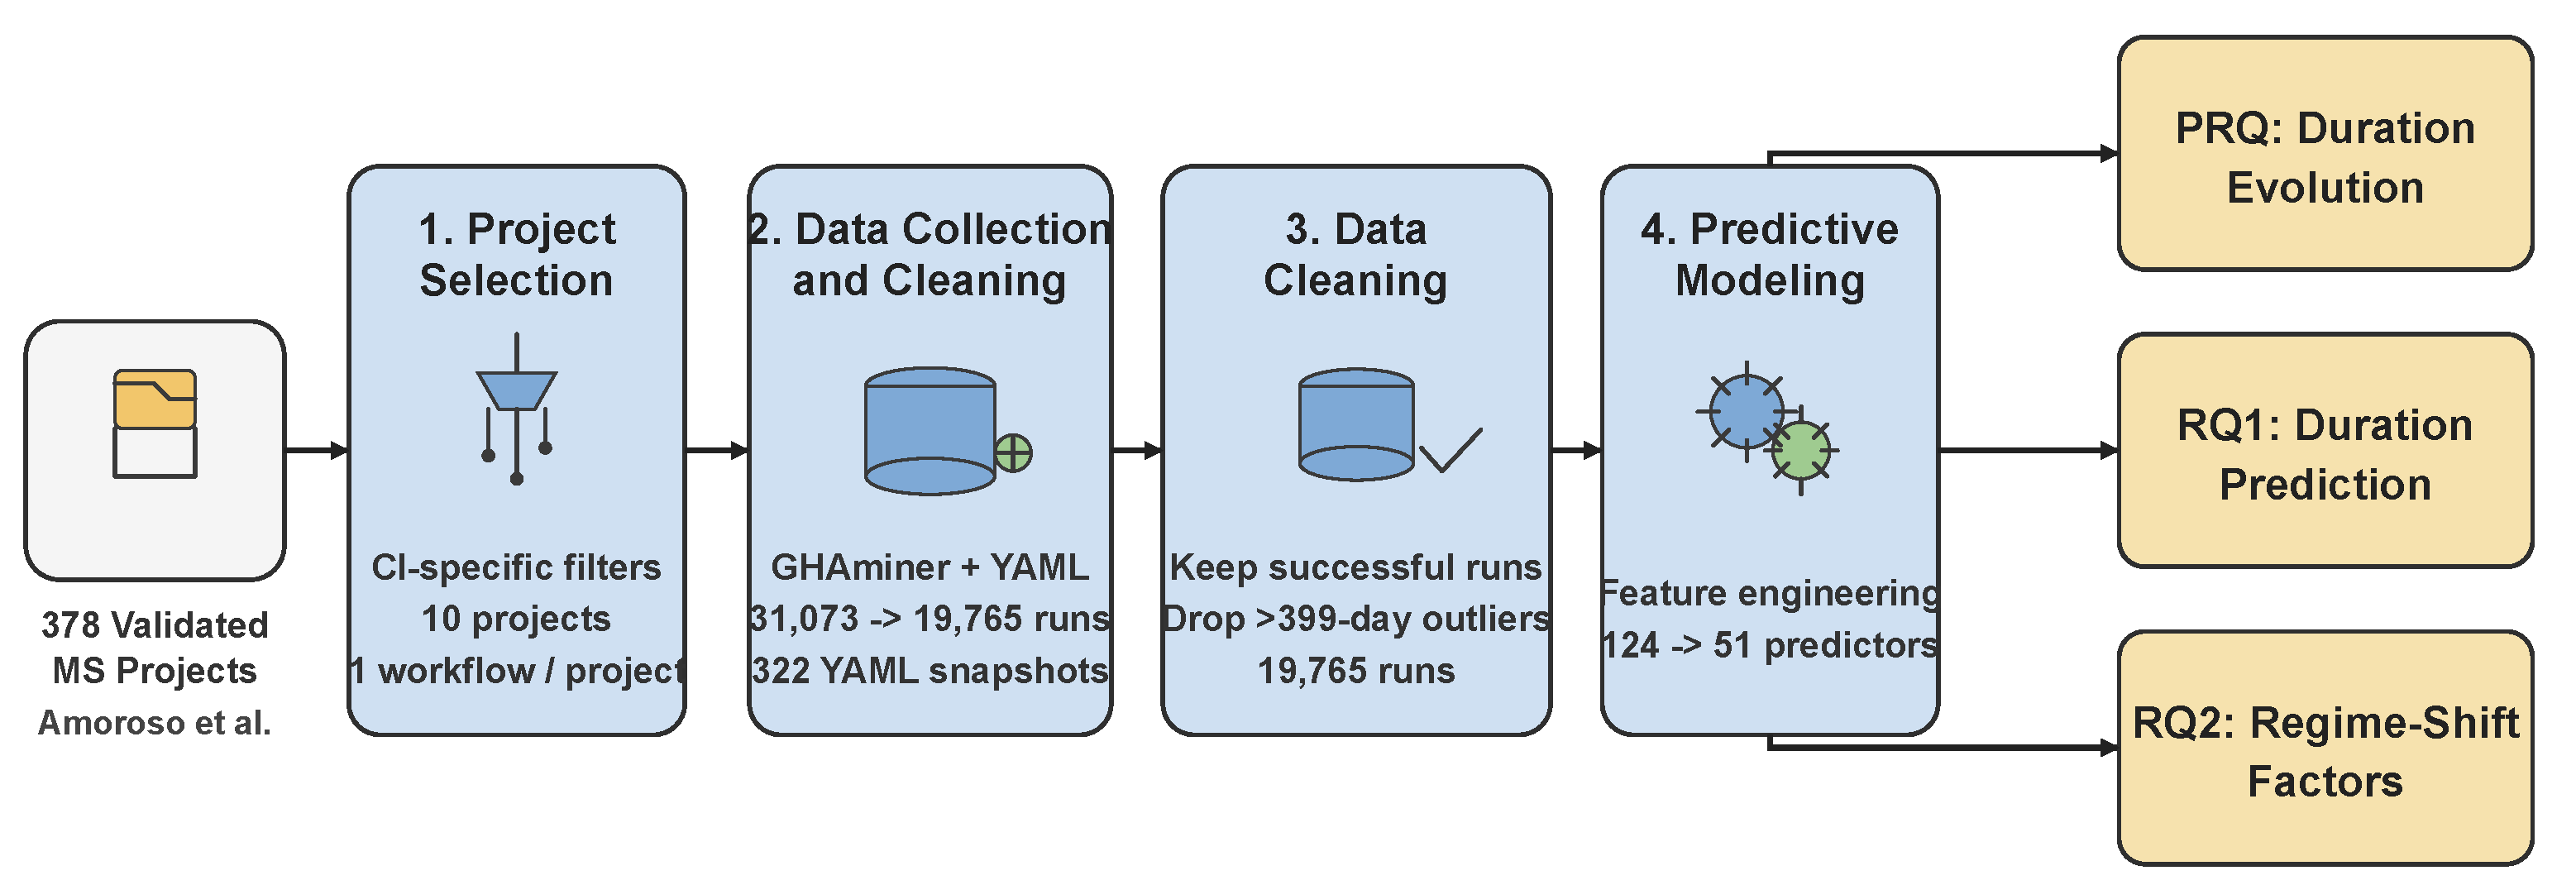
\includegraphics[width=0.8\textwidth]{figures/study_design.pdf}
\caption{Overview of the study design.}
\label{fig:study-design}
\end{figure*}

\subsection{Project Selection}
To select our candidate projects for this study, we first started with an existing dataset of 378 manually validated microservices-based GitHub repositories by Amoroso et al. \cite{amoroso2024dataset}. This dataset already retains active, non-trivial repositories by requiring recent activity, sufficient commits and contributors, at least one year of history, and the exclusion of toy or tutorial systems.
We then applied CI-specific filters adapted from prior GitHub Actions mining work \cite{bernardo2024gha}. A repository had to use \texttt{main} or \texttt{master} as its default branch, contain at least one YAML workflow in \texttt{.github/workflows}, provide at least 100 \texttt{push}- or \texttt{pull\_request}-triggered CI-relevant runs, and expose at least six months of workflow history. Applying these filters yielded 63 candidate projects, from which we randomly selected ten. We retained one CI-oriented workflow per project as the unit of analysis. Table~\ref{tab:projects_overview} reports the short labels used throughout the paper and summarizes the corresponding workflow histories before cleaning. Throughout the paper we use these short labels (for example, rust and radare2) to refer to the selected projects rather than to the programming languages or tools of the same name.

\begin{table}[!tbp]
\centering
%\scriptsize
    \fontsize{7.2}{8}\selectfont
    \tabcolsep=0.05cm
    \caption{Selected microservices-based projects summary.}
\label{tab:projects_overview}
\renewcommand{\arraystretch}{1.1}
\setlength{\tabcolsep}{3pt}
\begin{tabular}{llccccc}
\toprule
\textbf{Project} &
\makecell{\textbf{Primary}\\\textbf{Language}} &
\makecell{\textbf{Source}\\\textbf{Lines}\\\textbf{of Code}} &
\makecell{\textbf{Total}\\\textbf{Workflow}\\\textbf{Runs}} &
\makecell{\textbf{Workflow}\\\textbf{Lifetime}\\\textbf{(days)}} &
\makecell{\textbf{Median}\\\textbf{Duration}\\\textbf{(min)}} &
\makecell{\textbf{Duration}\\\textbf{MAD}\\\textbf{(min)}} \\
\midrule
ouds-android & Kotlin & 653k & 2,477 & 405.3 & 12.20 & 1.83 \\
bmad & Wolfram & 2.13M & 1,096 & 407.9 & 17.55 & 1.40 \\
ccpay & Java & 86.7k & 2,198 & 401.6 & 5.10 & 1.45 \\
FilterLists & C\# & 274k & 1,124 & 408.7 & 1.77 & 0.28 \\
daos & C & 1.29M & 8,672 & 419.2 & 31.78 & 7.89 \\
jod-yksilo-ui & TypeScript & 40.6k & 1,627 & 409.0 & 4.18 & 1.13 \\
m2os & Shell & 2.8k & 1,519 & 408.7 & 29.83 & 13.90 \\
Bruce & C++ & 116k & 781 & 323.7 & 5.03 & 0.33 \\
radare2 & C & 1.05M & 4,497 & 409.4 & 22.73 & 11.22 \\
rust & Rust & 80.5k & 7,082 & 410.1 & 7.79 & 2.66 \\
\bottomrule
\end{tabular}
\end{table}

\subsection{Data Collection}
We collected workflow histories with \textit{GHAminer} \cite{ghaminer}, an open source tool that extracts workflow-run, commit-level, pull-request, repository-level, and execution metadata from GitHub Actions repositories. In our case, this includes run timing and status information, workflow identifiers, commit and pull-request links, and repository context needed for downstream analysis. We also retrieved historical snapshots of each selected workflow YAML file and aligned each snapshot with the time interval in which it was active, so that YAML-derived metrics reflect the workflow definition that was actually executed. In addition, we retained the commit history and code-change patches associated with the collected runs to support later feature augmentation at the commit and patch levels. This collection phase yielded 31,073 workflow runs, 322 workflow-YAML snapshots, and 185,075 patch files across the ten selected project workflow histories.


\subsection{Data Cleaning}
To ensure data reliability, we applied a small set of cleaning steps before modeling. First, we retained only successful workflow runs, since they best reflect realized workflow duration rather than interrupted or failed executions, following prior work on CI performance analysis \cite{ghaleb2019longbuild,Wu2022DockerBuildDuration}. We then inspected extreme duration values and found runs approaching 400 days. These correspond to workflows that were triggered but never completed and were eventually removed under GitHub's retention policy \cite{githubretentiondocs}. We therefore filtered out all runs whose duration exceeded 399 days. After cleaning, the study dataset contained 19,765 successful workflow runs, which we use as the basis for the predictive analyses.

\subsection{Workflow Duration Prediction Modeling}
\noindent\underline{\textbf{\textit{Feature engineering.}}} We started from 58 per-run metrics collected directly with \textit{GHAminer} \cite{ghaminer}, covering workflow-run, repository, pull-request, and execution context available before prediction. We then leveraged the aligned historical workflow YAML snapshots to derive workflow-structure metrics, including caching, matrix, service, concurrency, runner, and step-complexity signals. Finally, we leveraged the commit history and associated patch data to derive additional metric groups capturing curated microservice file groups, commit timeline structure, and patch semantics spanning workflow edits, build and dependency changes, deployment changes, configuration changes, and test-related changes. In total, this process yielded 124 candidate predictors spanning temporal persistence, developer and repository context, workflow context, change activity and review context, workflow YAML structure, curated microservice file groups, commit timeline structure, and patch semantics. These predictors were inspired by prior work on time-aware CI prediction \cite{Atchison2017TravisTimeSeries,Saidani2020BuildFailureSearch,Wu2022DockerBuildDuration}, JIT-style change metrics \cite{Kamei2013JITQA,Saidani2020BuildFailureSearch}, workflow evolution and caching \cite{RostamiMazrae2026WorkflowEvolution,Hasan2026CachingEvolution}, and microservice deployment and coordination artifacts \cite{taibi2019continuous,karabey2021deployment,baresi2022docker,reile2022bunk8s,waseem2022decision}.

\noindent\underline{\textbf{\textit{Feature selection.}}} To reduce multicollinearity and redundancy among the engineered predictors, we applied a two-stage feature selection process inspired by prior work on build prediction \cite{Saidani2020BuildFailureSearch,Wu2022DockerBuildDuration}. First, we performed correlation-based clustering using the Spearman correlation coefficient. Predictors with pairwise correlation greater than 0.7 were grouped into clusters, and only one representative predictor from each cluster was retained. Next, we conducted redundancy analysis by regressing each remaining predictor against all others. Predictors with a coefficient of determination of at least 0.9 were treated as redundant and removed. This process reduced the 124 engineered candidate predictors to 51 non-redundant predictors used by the learned models. Table~\ref{tab:feature_summary_grouped} lists these retained predictors by category, type, and a short description.

\begin{table*}[!tp]
    \fontsize{6.5}{6.5}\selectfont
    \tabcolsep=0.1cm
\centering
\caption{Predictors retained after feature selection and used by the learned models.}
\label{tab:feature_summary_grouped}
\renewcommand{\arraystretch}{1.2}
\setlength{\tabcolsep}{4pt}
\begin{tabular}{p{2.6cm}p{5.3cm}p{0.8cm}p{7.2cm}}
\toprule
\textbf{Category} & \textbf{Feature Name} & \textbf{Type} & \textbf{Description} \\
\midrule
\multirow{1}{*}{\textbf{Temporal persistence}}
& \texttt{duration\_lag\_1} & N & Duration of the previous successful workflow run. \\
\midrule

\multirow{4}{*}{\textbf{Repository context}}
& \texttt{dependencies\_count} & N & Number of dependency declarations observed for the project snapshot. \\
& \texttt{gh\_sloc} & N & Repository source lines of code. \\
& \texttt{issuer\_name} & C & Encoded actor who triggered the workflow run. \\
& \texttt{project\_age\_days} & N & Project age in days since the first commit. \\
\midrule

\multirow{5}{*}{\textbf{Workflow context}}
& \texttt{branch} & C & Encoded branch name or branch category for the run. \\
& \texttt{gh\_is\_pr} & C & Indicates whether the run is associated with a pull request. \\
& \texttt{tests\_ran} & C & Indicates whether the workflow executed tests. \\
& \texttt{total\_jobs} & N & Number of jobs defined in the executed workflow. \\
& \texttt{workflow\_run\_count} & N & Repeat run count observed for the same workflow context. \\
\midrule

\multirow{2}{*}{\textbf{Workflow YAML}}
& \texttt{yaml\_has\_caching} & C & Indicates whether caching is configured in the active workflow YAML. \\
& \texttt{yaml\_max\_matrix\_size} & N & Maximum matrix size defined in the active workflow YAML. \\
\midrule

\multirow{5}{*}{\textbf{Change activity}}
& \texttt{dockerfile\_changed} & N & Number of changed Dockerfiles in the triggering revision. \\
& \texttt{gh\_commits\_on\_files\_touched} & N & Prior commits that touched the same changed files. \\
& \texttt{gh\_num\_pr\_comments} & N & Number of pull-request comments linked to the change. \\
& \texttt{gh\_other\_files} & N & Number of changed non-source, non-doc, non-test files. \\
& \texttt{gh\_test\_lines\_per\_kloc} & N & Test-line density normalized per KLOC. \\
\midrule

\multirow{6}{*}{\textbf{Microservice file groups}}
& \texttt{ft\_ms\_api\_contracts} & C & Indicates whether API-contract files were touched. \\
& \texttt{ft\_ms\_config\_data} & C & Indicates whether configuration or data files were touched. \\
& \texttt{ft\_ms\_frontend\_web} & C & Indicates whether frontend web files were touched. \\
& \texttt{ft\_ms\_jvm\_build\_and\_code} & C & Indicates whether JVM build or source files were touched. \\
& \texttt{ft\_ms\_scripts\_ops} & C & Indicates whether scripts or ops files were touched. \\
& \texttt{ft\_ms\_workflow\_yaml} & C & Indicates whether workflow YAML files were touched. \\
\midrule

\multirow{9}{*}{\textbf{Commit timeline}}
& \texttt{ct\_backend\_code\_touched} & C & Indicates whether backend source files were touched. \\
& \texttt{ct\_build\_manifest\_touched} & C & Indicates whether build manifest files were touched. \\
& \texttt{ct\_commit\_deletions} & N & Number of deleted lines in the triggering commits. \\
& \texttt{ct\_docs\_touched} & C & Indicates whether documentation files were touched. \\
& \texttt{ct\_k8s\_touched} & C & Indicates whether Kubernetes-related files were touched. \\
& \texttt{ct\_service\_like\_dirs\_touched} & C & Indicates whether service-like directories were touched. \\
& \texttt{ct\_shared\_component\_touched} & C & Indicates whether shared-component files were touched. \\
& \texttt{ct\_unique\_extensions} & N & Number of distinct file extensions in the change. \\
& \texttt{ct\_unique\_top\_dirs} & N & Number of distinct top-level directories touched. \\
\midrule

\multirow{6}{*}{\textbf{Code patch semantics}}
& \texttt{ps\_exception\_changed} & N & Count of exception-related edits in changed patches. \\
& \texttt{ps\_import\_changed\_lines} & N & Number of changed import/include lines. \\
& \texttt{ps\_logging\_changed} & N & Count of logging-related edits in changed patches. \\
& \texttt{ps\_patch\_comment\_changed\_lines} & N & Number of changed comment lines in patches. \\
& \texttt{ps\_patch\_files\_missing} & N & Number of patch files unavailable for semantic parsing. \\
& \texttt{ps\_todo\_fixme\_changed} & N & Count of changed TODO or FIXME markers. \\
\midrule

\multirow{2}{*}{\textbf{Workflow patch changes}}
& \texttt{ps\_workflow\_action\_version\_bumps} & N & Number of GitHub Action version updates in workflow patches. \\
& \texttt{ps\_workflow\_patch\_files} & N & Number of changed workflow patch files. \\
\midrule

\multirow{3}{*}{\textbf{Build and dependencies}}
& \texttt{ps\_build\_task\_lines\_changed} & N & Number of changed build-task lines. \\
& \texttt{ps\_dependency\_declaration\_changed} & N & Count of changed dependency declarations. \\
& \texttt{ps\_lockfile\_patch\_files} & N & Number of changed dependency lockfiles. \\
\midrule

\multirow{2}{*}{\textbf{Deployment patch changes}}
& \texttt{ps\_compose\_patch\_files} & N & Number of changed compose-related files. \\
& \texttt{ps\_docker\_base\_image\_changes} & N & Count of Docker base-image changes. \\
\midrule

\multirow{2}{*}{\textbf{Configuration patch changes}}
& \texttt{ps\_env\_key\_changed} & N & Count of changed environment-variable keys. \\
& \texttt{ps\_url\_or\_host\_changed} & N & Count of changed URLs or host strings. \\
\midrule

\multirow{4}{*}{\textbf{Test patch changes}}
& \texttt{ps\_assert\_changed} & N & Count of changed assertion statements. \\
& \texttt{ps\_skip\_test\_changed} & N & Count of changed skipped-test markers. \\
& \texttt{ps\_test\_case\_changed} & N & Count of changed test-case definitions. \\
& \texttt{ps\_test\_patch\_files} & N & Number of changed test-related patch files. \\
\bottomrule
\end{tabular}

\vspace{2mm}
\raggedright\footnotesize{N: Numeric, C: Categorical/binary indicator.}
\end{table*}
\noindent\underline{\textbf{\textit{Prediction setup.}}} We evaluate nine predictors under five expanding chronological splits per project. In each iteration, the model trained on the first 50\%, 60\%, 70\%, 80\%, and 90\% of the ordered history and tested on the immediately following 10\% segment. The compared predictors were the lag-1 baseline, Decision Tree (DT), k-Nearest Neighbors (KNN), Linear Regression (LR), Random Forest (RF), Gradient Boosting (SGB), Support Vector Regression (SVR), XGBoost (XGB), and HistGradientBoosting (HGB), following model families commonly used in CI prediction and software analytics studies \cite{Bisong2017BuildTimeModels,Arora2021AgileEffortRegression,Wu2022DockerBuildDuration}. Prior CI duration prediction studies use different comparison strategies, including random baselines and model-to-model comparisons \cite{Wu2022DockerBuildDuration,Bisong2017BuildTimeModels}. We use the duration of the previous successful workflow run as a lag-1 baseline because it provides a simple and strong temporal comparator for chronological workflow histories.


%\noindent\underline{\textbf{\textit{Evaluation metrics.}}} We report RMSE \ali{full name, then the abreviation, then citation. Fix everywhere}, MAE, $R^2$, and NRMSE, which are standard regression metrics in software engineering \ali{did you wrote the "-"? why? someone else wrote it? "software-engineering" -> "software engineering". Fix everywhere. } prediction studies \cite{Wu2022DockerBuildDuration,Arora2021AgileEffortRegression}. RMSE emphasizes large errors, MAE captures typical absolute error, and $R^2$ measures explained variance. Because workflows differ substantially in duration scale, we also report NRMSE, computed as $\mathrm{RMSE}/\sigma_y$, where $\sigma_y$ is the standard deviation of the test fold \cite{Ramakrishnan2020WebPerf}.

%\ali{full name, then the abreviation, then citation. Fix everywhere}\jasem{addressed}
% \ali{did you wrote the "-"? why? someone else wrote it? "software-engineering" -> "software engineering". Fix everywhere. }\jasem{addressed}
\noindent\underline{\textbf{\textit{Evaluation metrics.}}} We report Root Mean Square Error (RMSE), Mean Absolute Error (MAE), and coefficient of determination ($R^2$), which are widely used regression metrics in software engineering prediction studies \cite{Wu2022DockerBuildDuration,Arora2021AgileEffortRegression}. RMSE measures the square-root of the average squared prediction error and therefore gives more weight to larger errors. MAE measures the average absolute prediction error and captures the typical magnitude of the errors in the original unit of workflow duration. The coefficient of determination, $R^2$, measures the proportion of variance explained by the model. Since RMSE and MAE are scale-dependent and therefore not interpretable across projects, we additionally report the Normalized Root Mean Square Error (NRMSE), a scale-normalized version of RMSE that supports fairer comparison across projects with different duration scales \cite{Ramakrishnan2020WebPerf}. NRMSE is computed as $\mathrm{RMSE}/\sigma_y$, where $\sigma_y$ is the standard deviation of the test fold.



\section{Results}
In this section, we present the results of our study. We first address PQ by analyzing how CI workflow duration evolves over time in microservice-based projects.

\subsection{PQ: How does workflow duration evolve over time in microservices-based projects?}
%\noindent\underline{\textbf{\textit{Motivation.}}} Before building prediction models or explaining influential factors, we must first establish whether workflow duration behaves as a stable process or shifts over time. If histories contain substantial regime changes, then both predictive evaluation and interpretation should account for that temporal structure rather than assuming one uniform operating state.
\noindent\underline{\textbf{\textit{Motivation.}}} Prior studies suggest that CI duration may change over time rather than remain stable throughout a project's lifetime \cite{bernardo2024gha,ghaleb2023interplay}. In microservices-based projects, CI duration can be influenced by service boundaries, configuration-heavy artifacts, container and orchestration files, and integration-testing demands \cite{newman2021building,taibi2019continuous,baresi2022docker,reile2022bunk8s}. We therefore study whether CI duration in our sample remains stable over time or instead shifts between sustained duration levels.

\noindent\underline{\textbf{\textit{Approach.}}} We analyzed the 19,765 successful CI workflow runs from the 10 studied projects using a recursive change-point segmentation procedure based on Pettitt's test \cite{Pettitt1979}. We adopted this procedure to detect sustained shifts in duration. A split was retained only when it was statistically significant ($p < 0.01$), both resulting segments contained at least 75 runs, and the median duration changed by at least 10\%, so that the detected regions were both statistically supported and practically meaningful \cite{Mailhot2025RatingCurves}. The goal was to determine whether each workflow history behaves as one stable process or instead moves between distinct duration regimes over time.

\noindent\underline{\textbf{\textit{Results.}}} Figure~\ref{fig:prelim-regime-counts} reports how many stable regions were detected per project. Figures~\ref{fig:prq-example-no-shift}, \ref{fig:prq-example-three-shifts}, and \ref{fig:prq-example-five-shifts} illustrate representative histories with no accepted shift, an intermediate number of shifts, and the most segmented pattern. Table~\ref{tab:rq2-regime-cases} lists every accepted shift with median durations and percentage change.

\noindent\textbf{Finding~\#1: 7 out of 10 projects show at least one CI duration shift, with 18 accepted shifts between stable regions.}

Overall, the results reveal substantial heterogeneity in temporal structure. Three projects (Bruce, FilterLists, and ccpay) remain single-regime under the adopted thresholds, whereas ouds-android and rust split into five regions and radare2 into four. Figures~\ref{fig:prq-example-no-shift}, \ref{fig:prq-example-three-shifts}, and \ref{fig:prq-example-five-shifts} make this contrast visible: Bruce remains in one operating state, radare2 moves through a moderate multi-shift history, and ouds-android shows repeated upward transitions across five stable regions. The strongest upward jumps occur in ouds-android (about +68\%), radare2 (about +55\%), and daos (about +33\%), while the sharpest downward shifts appear in jod-yksilo-ui (about -36\%) and rust (about -33\%). A useful interpretation is that much of the apparent variability in these histories is not random fluctuation around one stable mean, but movement between locally stable operating states. This is why chronology matters: collapsing an entire workflow history into one average level can hide both sustained slowdowns and sustained speedups that are large enough to affect how prediction and explanation should be framed.

\noindent\textbf{Finding~\#2: Of the 18 duration shifts, 13 are increases and 5 are decreases.}

Across the 18 accepted shifts, 13 are increases and only 5 are decreases. This directional imbalance suggests that, in the studied microservices-based workflows, duration changes more often appear as sustained slowdowns than as sustained speedups. In practice, this means that once a workflow moves away from its earlier stable level, developers should be especially alert to the possibility that the boundary change has introduced a slower operating state rather than a short-lived spike. It also motivates treating increase and decrease transitions separately in the later local-factor analysis, since the two directions are not equally common in the observed histories.

% \ali{labels text ius unreadable}\jasem{addressed}
\begin{figure}[!tbp]
\centering
\includegraphics[width=\linewidth]{figures/prelim_stable_region_counts.png}
\caption{Number of stable regions detected in each project's CI history.}
\label{fig:prelim-regime-counts}
\end{figure}

%\ali{labels text ius unreadable}\jasem{addressed}
\begin{figure}[!t]
\centering
\includegraphics[width=\linewidth]{figures/prq_example_bruce_no_shift.png}
\caption{Example of a CI workflow history with no accepted regime shift (Bruce).}
\label{fig:prq-example-no-shift}
\end{figure}

% \ali{labels text ius unreadable}\jasem{addressed} \ali{remove the text in top of the figure. Add it in to the caption if needed, or removed it if redundant with the the caption}\jasem{addressed}
\begin{figure}[!t]
\centering
\includegraphics[width=\linewidth]{figures/prq_example_radare2_three_shifts.png}
\caption{Example of a CI workflow history with three accepted regime shifts (radare2).}
\label{fig:prq-example-three-shifts}
\end{figure}

%\ali{labels text ius unreadable}\jasem{addressed}
\begin{figure}[!t]
\centering
\includegraphics[width=\linewidth]{figures/prq_example_ouds_android_five_regions.png}
\caption{Example of a CI workflow history with five stable regions (ouds-android).}
\label{fig:prq-example-five-shifts}
\end{figure}

\subsection{RQ1: Could workflow duration be accurately predicted in microservices-based projects?}
\noindent\underline{\textbf{\textit{Motivation.}}} After establishing in PQ that workflow duration is often regime-structured, the next step is to test how accurately future duration can be predicted under a chronology-preserving setup. This determines whether the available repository, workflow, and temporal signals contain enough information to outperform a simple lag-based baseline in realistic microservices-based CI settings.

\noindent\underline{\textbf{\textit{Approach.}}} RQ1 evaluates nine predictors over the five expanding windows described in Section~3.4. In addition to the lag-1 baseline, we compare DT, KNN, LR, RF, SGB, SVR, XGB, and HGB. To improve robustness, the learned models retain globally screened lag-history features, clip each training fold to the 1st--99th percentile range before fitting, and apply target-side clipping during training; the tree and kernel families also use conservative shallow/regularized settings to reduce overfitting.

\noindent\underline{\textbf{\textit{Results.}}} Table~\ref{tab:rq1-rmse} summarizes predictive performance for all models across the ten workflows, using RMSE, MAE, $R^2$, and NRMSE under five expanding chronological windows.

%\ali{"Observation" -> "Finding"}\jasem{addressed}
\noindent\textbf{Finding~\#3: HGB achieves the highest global average $R^2$ and NRMSE across the ten studied projects}

Overall, the revised setup produces a much stronger and more stable picture than the earlier run. The best learned model now beats the lag-1 baseline in all ten workflows on RMSE, NRMSE, and $R^2$, eliminating the previous cases in which inertia remained the strongest predictor. HGB delivers the best global average results ($R^2 \approx 0.15$, NRMSE $\approx 0.90$) and is the best NRMSE model for ouds-android, bmad, m2os, and radare2. Other winners remain workflow-specific: SGB is best on ccpay and Bruce, RF on FilterLists and rust, LR on daos, and SVR on jod-yksilo-ui. Seven workflows now attain positive best-model $R^2$ values (FilterLists, daos, jod-yksilo-ui, m2os, Bruce, radare2, and rust), while the remaining three retain negative $R^2$ but improve substantially over the baseline. The clearest success case remains rust, where RF reduces RMSE from about 149 to 77 and raises $R^2$ from about $-0.57$ to $0.57$; ouds-android also changes from baseline-dominated to HGB-led, with RMSE dropping from about 217 to 168 and NRMSE from 1.37 to 1.07. The practical implication is that chronology-aware learned models can consistently outperform simple temporal persistence when robust training and richer duration-history signals are included, but the best-performing family is still project-dependent.

Because the RMSE-best learner is not always the $R^2$-best learner (e.g., bmad favors HGB by RMSE/NRMSE but LR by $R^2$), RQ2 reuses the per-project $R^2$-best model for local explanation so that the regime-shift windows are analyzed with the strongest variance-explaining learner available for each project.

%\ali{write more descriptive captions: example "Prediction performance across projects for CI workflow duration using multiple predictive models. Fix everywhere"}\jasem{addressed}
\begin{table}[!tbp]
    \fontsize{6}{6.5}\selectfont
    \tabcolsep=0.01cm
\centering
%\scriptsize
\renewcommand{\arraystretch}{1.1}
\setlength{\tabcolsep}{3pt}
\caption{Prediction performance across projects for CI workflow duration using multiple predictive models.}
\label{tab:rq1-rmse}
\begin{tabular}{llccccccccc}
\toprule
\textbf{Project} & \textbf{Metric} &
\textbf{Baseline} &
\textbf{DT} & \textbf{KNN} & \textbf{LR} &
\textbf{RF} & \textbf{SGB} & \textbf{SVR} & \textbf{XGB} & \textbf{HGB} \\
\midrule
\multirow{4}{*}{ouds-android} & RMSE & 217 & 176 & 184 & 213 & 174 & 171 & 205 & 172 & \textbf{168} \\
  & MAE & 145 & 125 & 126 & 157 & 117 & 118 & 146 & 118 & \textbf{117} \\
  & $R^2$ & -0.891 & -0.259 & -0.388 & -0.941 & -0.223 & -0.178 & -0.747 & -0.189 & \textbf{-0.142} \\
  & NRMSE & 1.370 & 1.118 & 1.174 & 1.371 & 1.103 & 1.082 & 1.313 & 1.087 & \textbf{1.065} \\
\midrule
\multirow{4}{*}{bmad} & RMSE & 78 & 69 & 69 & 64 & 69 & 65 & 77 & 65 & \textbf{64} \\
  & MAE & 51 & 45 & 46 & 41 & 45 & 41 & 53 & 42 & \textbf{40} \\
  & $R^2$ & -0.624 & -0.332 & -0.367 & \textbf{-0.121} & -0.377 & -0.165 & -0.655 & -0.190 & -0.132 \\
  & NRMSE & 1.259 & 1.144 & 1.153 & 1.052 & 1.146 & 1.066 & 1.274 & 1.075 & \textbf{1.050} \\
\midrule
\multirow{4}{*}{ccpay} & RMSE & 36 & 34 & 31 & 29 & 29 & \textbf{29} & 36 & 30 & 29 \\
  & MAE & 29 & 28 & 26 & 24 & 25 & \textbf{24} & 29 & 25 & 24 \\
  & $R^2$ & -0.785 & -0.575 & -0.333 & -0.134 & -0.154 & \textbf{-0.125} & -0.761 & -0.202 & -0.146 \\
  & NRMSE & 1.321 & 1.236 & 1.141 & 1.055 & 1.064 & \textbf{1.052} & 1.308 & 1.086 & 1.063 \\
\midrule
\multirow{4}{*}{FilterLists} & RMSE & 58 & 49 & 35 & 67 & \textbf{33} & 38 & 37 & 37 & 36 \\
  & MAE & 41 & 33 & 22 & 45 & \textbf{20} & 22 & 23 & 23 & 20 \\
  & $R^2$ & -0.892 & -0.464 & 0.299 & -1.604 & \textbf{0.375} & 0.143 & 0.235 & 0.147 & 0.241 \\
  & NRMSE & 1.359 & 1.130 & 0.794 & 1.569 & \textbf{0.764} & 0.870 & 0.853 & 0.857 & 0.823 \\
\midrule
\multirow{4}{*}{daos} & RMSE & 1018 & 1044 & 1129 & \textbf{942} & 1016 & 948 & 1091 & 959 & 950 \\
  & MAE & 655 & 656 & 710 & 599 & 619 & 594 & 680 & 596 & \textbf{591} \\
  & $R^2$ & 0.304 & 0.268 & 0.148 & \textbf{0.407} & 0.312 & 0.400 & 0.208 & 0.386 & 0.396 \\
  & NRMSE & 0.831 & 0.853 & 0.921 & \textbf{0.769} & 0.828 & 0.773 & 0.888 & 0.782 & 0.776 \\
\midrule
\multirow{4}{*}{jod-yksilo-ui} & RMSE & 78370 & 54653 & 55148 & 54502 & 55105 & 54512 & \textbf{54034} & 54766 & 54510 \\
  & MAE & 16276 & 10249 & \textbf{8129} & 8819 & 8180 & 8774 & 8337 & 8602 & 8561 \\
  & $R^2$ & -1.036 & -0.189 & 0.004 & 0.075 & 0.018 & 0.080 & \textbf{0.088} & -0.174 & 0.057 \\
  & NRMSE & 1.421 & 1.057 & 0.994 & 0.956 & 0.986 & 0.953 & \textbf{0.943} & 1.057 & 0.966 \\
\midrule
\multirow{4}{*}{m2os} & RMSE & 1296 & 1010 & 1009 & 892 & 1027 & 898 & 983 & 892 & \textbf{882} \\
  & MAE & 800 & 675 & 620 & 614 & 656 & 606 & 609 & 594 & \textbf{591} \\
  & $R^2$ & -0.394 & 0.215 & 0.212 & 0.337 & 0.183 & 0.354 & 0.256 & 0.364 & \textbf{0.371} \\
  & NRMSE & 1.162 & 0.873 & 0.876 & 0.800 & 0.894 & 0.790 & 0.852 & 0.785 & \textbf{0.780} \\
\midrule
\multirow{4}{*}{Bruce} & RMSE & 47 & 45 & 43 & 81 & 42 & 42 & 48 & \textbf{42} & 43 \\
  & MAE & \textbf{29} & 31 & 30 & 63 & 29 & 29 & 34 & 30 & 30 \\
  & $R^2$ & -0.253 & -0.165 & -0.060 & -5.813 & -0.002 & \textbf{0.011} & -0.327 & 0.009 & -0.024 \\
  & NRMSE & 1.095 & 1.066 & 1.015 & 1.855 & 0.989 & \textbf{0.984} & 1.136 & 0.986 & 1.000 \\
\midrule
\multirow{4}{*}{radare2} & RMSE & 1582 & 1051 & 1069 & 1131 & 978 & 957 & 1111 & 953 & \textbf{953} \\
  & MAE & 1263 & 741 & 752 & 806 & 666 & 651 & 784 & 644 & \textbf{642} \\
  & $R^2$ & -0.819 & 0.215 & 0.189 & 0.092 & 0.322 & 0.350 & 0.121 & 0.355 & \textbf{0.356} \\
  & NRMSE & 1.342 & 0.882 & 0.898 & 0.950 & 0.817 & 0.800 & 0.933 & 0.797 & \textbf{0.796} \\
\midrule
\multirow{4}{*}{rust} & RMSE & 149 & 82 & 86 & 92 & \textbf{77} & 84 & 90 & 80 & 81 \\
  & MAE & 101 & \textbf{49} & 53 & 66 & 49 & 53 & 61 & 50 & 51 \\
  & $R^2$ & -0.566 & 0.524 & 0.433 & 0.330 & \textbf{0.568} & 0.469 & 0.373 & 0.541 & 0.529 \\
  & NRMSE & 1.249 & 0.683 & 0.727 & 0.790 & \textbf{0.644} & 0.708 & 0.771 & 0.666 & 0.674 \\
\midrule
\multirow{4}{*}{\textbf{Global Avg}} & RMSE & 8285 & 5821 & 5880 & 5801 & 5855 & 5774 & \textbf{5771} & 5800 & 5772 \\
  & MAE & 1939 & 1263 & 1051 & 1123 & \textbf{1041} & 1091 & 1075 & 1072 & 1067 \\
  & $R^2$ & -0.596 & -0.076 & 0.014 & -0.737 & 0.102 & 0.134 & -0.121 & 0.105 & \textbf{0.151} \\
  & NRMSE & 1.241 & 1.004 & 0.969 & 1.117 & 0.924 & 0.908 & 1.027 & 0.918 & \textbf{0.899} \\
\bottomrule
\end{tabular}
\end{table}

\subsection{RQ2: Which factors are associated with workflow duration shifts in microservices-based projects?}
\noindent\underline{\textbf{\textit{Motivation.}}} PQ shows that the studied histories are often divided into stable regions separated by substantial shifts in median duration. A global run-level explanation does not directly answer what is associated with those transitions. We therefore focus on the regime-shift events themselves and ask which factors recur when workflows move upward into slower states or downward into faster ones.

\noindent\underline{\textbf{\textit{Approach.}}} We analyzed all 18 accepted duration shifts identified in PQ. For each shift, we defined a local test window around the transition using the last 25\% of runs from the earlier stable region and the first 25\% of runs from the later stable region, with a balanced size on both sides. We then selected, for each project, the RQ1 model with the best $R^2$, trained it on all runs observed before the local test window, and computed permutation importance on that shift-area window. This design keeps the analysis local to the transition itself while avoiding information leakage from runs that occur after the shift. We finally summarized the resulting local importance rankings separately for increase and decrease shifts. Table~\ref{tab:rq2-regime-cases} lists the duration regime-shift cases analyzed in this step.

\begin{figure}[!htbp]
\centering
\includegraphics[width=\linewidth]{figures/rq2_shift_window_example_bmad.png}
\caption{Example CI workflow history highlighting the areas of around two duration shifts.}
\label{fig:rq2-shift-window-example}
\end{figure}

\begin{table}[!htbp]
\centering
    \fontsize{7}{8}\selectfont
    \tabcolsep=0.01cm
    %\scriptsize
\caption{Accepted regime-shift cases analyzed in RQ2.}
\label{tab:rq2-regime-cases}
%\renewcommand{\arraystretch}{1.08}
\setlength{\tabcolsep}{3pt}
\resizebox{\columnwidth}{!}{%
\begin{tabular}{lcccc}
\toprule
\textbf{Project} & \textbf{Regime Shift} & \textbf{Regime 1 Median (min)} & \textbf{Regime 2 Median (min)} & \textbf{Change (\%)} \\
\midrule
bmad & R1$\rightarrow$R2 & 18.41 & 16.08 & \cellcolor{red!18}-12.63 \\
bmad & R2$\rightarrow$R3 & 16.08 & 18.98 & \cellcolor{green!18}17.98 \\
daos & R1$\rightarrow$R2 & 29.57 & 39.47 & \cellcolor{green!18}33.48 \\
jod-yksilo-ui & R1$\rightarrow$R2 & 4.12 & 4.60 & \cellcolor{green!18}11.74 \\
jod-yksilo-ui & R2$\rightarrow$R3 & 4.60 & 2.93 & \cellcolor{red!18}-36.23 \\
m2os & R1$\rightarrow$R2 & 27.59 & 32.08 & \cellcolor{green!18}16.28 \\
m2os & R2$\rightarrow$R3 & 32.08 & 36.22 & \cellcolor{green!18}12.88 \\
ouds-android & R1$\rightarrow$R2 & 5.87 & 9.88 & \cellcolor{green!18}68.32 \\
ouds-android & R2$\rightarrow$R3 & 9.88 & 11.25 & \cellcolor{green!18}13.92 \\
ouds-android & R3$\rightarrow$R4 & 11.25 & 13.75 & \cellcolor{green!18}22.22 \\
ouds-android & R4$\rightarrow$R5 & 13.75 & 16.73 & \cellcolor{green!18}21.70 \\
radare2 & R1$\rightarrow$R2 & 20.66 & 31.93 & \cellcolor{green!18}54.58 \\
radare2 & R2$\rightarrow$R3 & 31.93 & 39.35 & \cellcolor{green!18}23.23 \\
radare2 & R3$\rightarrow$R4 & 39.35 & 29.63 & \cellcolor{red!18}-24.69 \\
rust & R1$\rightarrow$R2 & 11.37 & 12.72 & \cellcolor{green!18}11.95 \\
rust & R2$\rightarrow$R3 & 12.72 & 10.67 & \cellcolor{red!18}-16.18 \\
rust & R3$\rightarrow$R4 & 10.67 & 7.20 & \cellcolor{red!18}-32.50 \\
rust & R4$\rightarrow$R5 & 7.20 & 8.18 & \cellcolor{green!18}13.66 \\
\bottomrule
\end{tabular}
}
\end{table}

\noindent\underline{\textbf{\textit{Results.}}} Table~\ref{tab:rq2-increase-top10} ranks features for the 13 median-duration \emph{increase} events; Table~\ref{tab:rq2-decrease-top10} ranks features for the five \emph{decrease} events using mean rank, median rank, and average normalized importance.

\noindent\textbf{Finding~\#4: Duration increase shifts are led by testing, persistence, and repository-change signals, whereas decrease shifts are led more by lockfile, patch-semantic, and workflow/configuration context.}

Overall, the feature rankings change noticeably when the models are trained only on the history preceding the shift-area window and then evaluated directly on the runs nearest the shift. On the increase side, \texttt{tests\_ran} is now the clearest leading signal, followed by \texttt{duration\_lag\_1}, \texttt{ps\_lockfile\_patch\_files}, \texttt{gh\_other\_files}, and \texttt{ct\_commit\_deletions}. This suggests that upward transitions are associated less with one broad maturity/context factor and more with a mix of execution intensity, short-term temporal persistence, and nearby repository or dependency churn. On the decrease side, the rankings are still based on only five events, but the most recurrent signals now center on \texttt{ps\_lockfile\_patch\_files}, \texttt{ps\_patch\_comment\_changed\_lines}, \texttt{ft\_ms\_frontend\_web}, \texttt{ft\_ms\_config\_data}, and \texttt{ft\_ms\_workflow\_yaml}. This asymmetry remains important: in our data, speedups are not simply slowdowns with the sign reversed, but are associated more with a smaller set of local configuration and patch-related factors. Because the decrease side contains only five events, these patterns should still be read as directional evidence rather than as a universal ranking.

We further investigate workflow runs around the regime shift areas to interpret these shift-local feature signals. For instance, in \texttt{bmad} (\texttt{R1}$\rightarrow$\texttt{R2}), the median duration decreased from 18.41 to 16.08 minutes ($-12.63\%$), and the boundary run fell from 17.07 to 15.07 minutes. The boundary commit reduced the PyTao workflow to a filtered subset of tests \cite{bmadPytaoScopeReductionPR}, and the linked discussion noted that \textit{"The pytao test job is about 3 minutes more than the current `master' CI builds"} while normal builds were \textit{"reduced by maybe 2 minutes at times (due to the increase in parallel `make' jobs)"} \cite{bmadPytaoDurationComment}. By contrast, in \texttt{m2os} (\texttt{R2}$\rightarrow$\texttt{R3}), the median duration increased from 32.08 to 36.22 minutes ($+12.88\%$), and the boundary run rose from 31.68 to 63.85 minutes. The corresponding boundary change refreshed the base container images used by the workflow, so subsequent CI runs built on a different container base than before \cite{m2osBaseImageUpdatePR}. This is consistent with the slower post-shift regime.


\begin{table}[!htbp]
\centering
\scriptsize
\caption{Top 10 features associated with CI duration increase shifts.}
\label{tab:rq2-increase-top10}
\renewcommand{\arraystretch}{1.08}
\setlength{\tabcolsep}{2pt}
\resizebox{\columnwidth}{!}{%
\begin{tabular}{clccc}
\toprule
\textbf{Rank} & \textbf{Feature} & \textbf{Mean Rank} & \textbf{Median Rank} & \textbf{Avg. Norm. Score (\%)} \\
\midrule
1 & \texttt{tests\_ran} & 1.00 & 1.00 & 29.32 \\
2 & \texttt{duration\_lag\_1} & 12.54 & 6.00 & 13.27 \\
3 & \texttt{ps\_lockfile\_patch\_files} & 10.33 & 7.00 & 11.35 \\
4 & \texttt{gh\_other\_files} & 10.42 & 6.00 & 9.54 \\
5 & \texttt{ct\_commit\_deletions} & 10.31 & 7.00 & 9.31 \\
6 & \texttt{branch} & 16.10 & 22.00 & 8.22 \\
7 & \texttt{gh\_commits\_on\_files\_touched} & 15.50 & 13.50 & 8.10 \\
8 & \texttt{project\_age\_days} & 15.23 & 12.00 & 7.31 \\
9 & \texttt{window\_avg\_7} & 14.15 & 12.00 & 6.89 \\
10 & \texttt{gh\_test\_lines\_per\_kloc} & 18.45 & 16.50 & 5.10 \\
\bottomrule
\end{tabular}
}
\end{table}

\begin{table}[!htbp]
\centering
    \fontsize{9}{10}\selectfont
    \tabcolsep=0.01cm
    %\scriptsize
\caption{Top 10 features associated with CI duration decrease shifts}
\label{tab:rq2-decrease-top10}
\renewcommand{\arraystretch}{1.08}
\setlength{\tabcolsep}{2pt}
\resizebox{\columnwidth}{!}{%
\begin{tabular}{clccc}
\toprule
\textbf{Rank} & \textbf{Feature} & \textbf{Mean Rank} & \textbf{Median Rank} & \textbf{Avg. Norm. Score (\%)} \\
\midrule
1 & \texttt{ps\_lockfile\_patch\_files} & 11.67 & 2.00 & 22.30 \\
2 & \texttt{ps\_patch\_comment\_changed\_lines} & 13.60 & 11.00 & 17.09 \\
3 & \texttt{ft\_ms\_frontend\_web} & 8.00 & 3.00 & 13.20 \\
4 & \texttt{ft\_ms\_config\_data} & 16.80 & 20.00 & 11.56 \\
5 & \texttt{ft\_ms\_workflow\_yaml} & 7.30 & 9.00 & 8.47 \\
6 & \texttt{branch} & 16.20 & 16.00 & 7.25 \\
7 & \texttt{project\_age\_days} & 14.40 & 14.00 & 6.38 \\
8 & \texttt{duration\_lag\_1} & 5.80 & 5.00 & 5.97 \\
9 & \texttt{gh\_is\_pr} & 15.40 & 21.00 & 4.28 \\
10 & \texttt{tests\_ran} & 6.00 & 6.00 & 3.65 \\
\bottomrule
\end{tabular}
}
\end{table}

\begin{figure}[!htbp]
\centering
\includegraphics[width=\linewidth]{figures/rq2_increase_shift_feature_heatmap.png}
\caption{Top influential feature importance heatmap for duration increase shifts across projects}
\label{fig:rq2-increase-feature-heatmap}
\end{figure}

\begin{figure}[!htbp]
\centering
\includegraphics[width=\linewidth]{figures/rq2_decrease_shift_feature_heatmap.png}
\caption{Top influential feature importance heatmap for duration decrease shifts across projects}
\label{fig:rq2-decrease-feature-heatmap}
\end{figure}

\section{Threats to Validity}
\noindent\textbf{Construct validity.} Our feature families are proxies for workflow, repository, and change phenomena rather than direct measurements of every engineering decision. For example, curated microservice file groups and patch-semantic counters approximate coordination and configuration work, but they cannot fully capture developer intent. The project-level filters themselves are a construct choice: we adapted them from prior GitHub Actions mining work \cite{bernardo2024gha} and applied them uniformly to all candidate repositories, but different thresholds on CI activity or history length would yield a different (though overlapping) project pool. A second construct threat is that we analyze one CI-oriented workflow per project, which is a deliberate scoping choice so that results are comparable across projects, but which means the observed behavior may not represent every workflow inside the same repository. We mitigate part of the remaining drift by aligning workflow-configuration features to the YAML snapshot active at each run, so that features describing the workflow definition move with the workflow rather than being taken from a single static version.

\noindent\textbf{Internal validity.} GitHub Actions retention policies limit how much historical workflow data can be observed, so the analyzed histories cover roughly one year rather than multiple years \cite{githubretentiondocs}. We mitigate temporal leakage by using expanding chronological splits, but observational data still prevent causal claims about why a duration change happened. The PQ results also depend on the Pettitt-based segmentation thresholds (\(p < 0.01\), at least 75 runs per resulting segment, and a median-duration change of at least 10\%). We fixed these thresholds a priori rather than tuning them on the data, and we report them explicitly so that the segmentation is reproducible, but a stricter or looser setting would change how many regimes are detected. Another internal-validity consideration is that the direction-specific patch counters were merged into a single ``changed'' form in the final rerun; this simplifies interpretation but loses the separation between additions and removals.

\noindent\textbf{External validity.} The study covers ten microservices-based projects and one CI-oriented workflow per project. Although the repositories were drawn from the validated microservices dataset of Amoroso et al.\ \cite{amoroso2024dataset} and then filtered for non-trivial GitHub Actions usage, the study is not intended as a statistical claim about all microservices systems: our CI-activity and history-length filters exclude smaller or very young repositories by design, and the per-project sample sizes are not balanced. The results should therefore be read as empirical evidence on ten sufficiently active microservices workflows, and replication on larger and more diverse samples (including multiple workflows per repository and longer histories) is needed before generalizing the observed patterns.

\noindent\textbf{Conclusion validity.} Raw RMSE and MAE values are scale-dependent, so cross-project averages of those metrics must be interpreted cautiously. We therefore also report NRMSE and keep the lag-1 baseline as a strong temporal comparator, which is the main anchor for practical improvement rather than absolute error magnitudes. In RQ2, local permutation importance reveals predictive influence around the fitted regime-shift windows, but it does not by itself imply causal importance. The 18 accepted regime-shift events are also not evenly split (13 increases vs.\ 5 decreases), so decrease-side rankings are supported by fewer cases and are more sensitive to individual transitions; we therefore summarize rankings with medians and mean ranks and avoid causal wording for either direction.

\section{Takeaway and Implications}
In this section, we summarize the main insights from our study and discuss their implications for practitioners and researchers.

\subsection{For Practitioners}

\textbf{(1) MS Developers should treat a sudden CI slowdown as a possible shift to a new duration regime rather than as a one-off anomaly.}
PQ shows that 7 of the 10 studied projects experienced at least one meaningful duration shift, with 18 accepted shifts overall, and 13 of them were increases. This means that once a workflow becomes slower, it is more likely to stay slower for some time than to immediately return to its earlier level. In practice, teams should inspect the boundary run and the boundary commit whenever a visible slowdown appears, because that boundary may mark the start of a new operating state for the workflow rather than a random fluctuation.

\textbf{(2) When workflow duration changes, developers should inspect the factors most associated with the direction of the change.}
RQ2 shows that duration increases are more associated with testing, short-term persistence, and nearby repository-change signals, whereas decreases are more associated with lockfile, patch-semantic, and workflow/configuration context. A useful practical response is therefore direction-specific: when a workflow slows down, first inspect added or expanded tests, recent duration history, and nearby repository churn; when it speeds up, first inspect dependency, patch, and workflow-configuration changes. RQ1 further suggests that teams should monitor workflow duration with project-specific models or baselines, since the best predictor was not the same across projects.

\subsection{For Researchers}

\textbf{(1) Researchers should study CI duration shifts explicitly, at larger scale, rather than assuming that workflow duration is stable over time.}
PQ shows that workflow duration in microservices-based CI is often structured by sustained shifts rather than one stable average level. This opens several directions for future work: measuring how often such shifts occur in larger and more diverse samples, studying whether increase shifts are consistently more common than decrease shifts, and qualitatively analyzing the boundary commits and workflow edits that trigger these transitions. In other words, duration shifts themselves should be treated as an empirical object of study, not only as noise around a prediction target.

\textbf{(2) Researchers should model workflow duration locally and directionally, not only with one global explanation.}
RQ1 and RQ2 together show that duration can be predicted better than a simple lag-based baseline, but that the best model remains project-specific and that increase and decrease shifts are associated with different local signals. This suggests that future studies should move beyond one global model over the full workflow history and instead examine local transition windows, direction-aware explanations, and eventually causal analyses of why particular boundary changes lead to slower or faster sustained regimes.


\section{Conclusion}
This paper studied GitHub Actions workflow duration in microservices-based projects through temporal analysis, chronological prediction, and local shift explanation. We found that workflow duration is often not stable over time: 7 of the 10 studied projects exhibited at least one meaningful duration shift, yielding 18 accepted shifts overall. We further found that learned models consistently improved over a strong lag-1 baseline, although the best-performing model remained project-specific. Finally, our local shift analysis showed that duration increases are more associated with testing, persistence, and nearby repository-change signals, whereas decreases are more associated with lockfile, patch-semantic, and workflow/configuration context. These findings highlight a broader challenge in understanding CI for microservices-based systems. Workflow duration is not merely noisy; it can reorganize into a new stable level after specific boundary changes, and those transitions are not explained equally well by one global model or one universal factor. This raises an important question for future work: how can CI systems detect, explain, and respond to duration shifts early enough that a sustained slowdown is treated as a diagnosable transition rather than simply accepted as the new baseline? Answering this question is important for building CI pipelines that remain predictable, efficient, and trustworthy as microservices-based projects evolve.


\bibliographystyle{IEEEtran}
\bibliography{refs}

\balance

\end{document}
\\
